\chapter{OpenCL}

\section{Wprowadzenie}
OpenCL (Open Computing Language) jest standardem tworzenia oprogramowania stworzonym przez Khronos Group, który powstał w celu wsparcia w tworzeniu oprogramowania z wykorzystaniem mocy zarówno współczesnych kart graficznych (GPU) jak i procesorów (CPU). Jedną z głównych zalet OpenCL jest otwartość standardu, co umożliwia wykorzystanie technologii opierając się o sprzęt wielu producentów (np. Nvidia, AMD, Intel).

\section{Składniki środowiska OpenCL}
Idea funkcjonowania platformy OpenCL została przedstawiona na rysunku 2.1. \\
\begin{figure}[h]
\centering
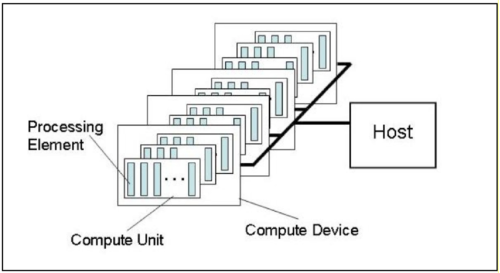
\includegraphics[width=0.8\textwidth]{figures/opencl_platform_model.png}
\caption{Model platformy OpenCL.\protect\footnotemark}%
\label{rys:OpenCL Platform Model}
\end{figure}
\footnotetext{Źródło: http://pclab.pl/zdjecia/artykuly/miekrzy/catalyst8\_12/host.png}
Środowisko składa się z hosta – „gospodarza”, nakazujacego wykonanie konkretnego ciagu instrukcji urządzeniom obliczeniowym (Compute Device). Każde urządzenie posiada własny zestaw jednostek przetwarzających, na których istrukcje są wykonywane.

\section{Architektura OpenCL}
Architektura OpenCL składa się z trzech zasadniczych części: specyfikacji języka, API platformy i API czasu wykonania. Specyfikacja języka OpenCL definiuje składnię programów i kerneli\footnote{funkcja wykonywana na urządzeniu, korzystajaca korzystajaca z jego zasobów}, które oparte są na zmodyfikowanym standardzie ISO C99, zawierającym część dodanych, zmienionych oraz usuniętych słów kluczowych a takze rozszerzeniu standardu np. poprzez dodanie wsparcie dla przetwarzania równoległego. \\
API platformy umożliwia hostowi uruchamianie stworzonych kerneli na urządzeniach obliczeniowych. Realizuje ono również koncepcję kontekstu. Kontekst jest kontenerem grupującym urządzenie z przeznaczoną dla niego zawartością pamięci oraz kolejkami zadań. Przy pomocy API platformy realizowane jest przekazywanie danych między hostem a urządzeniem obliczeniowym. \\
API czasu wykonania wykorzystuje dostarczone przez platformę konteksty do kontrolowania kompatybilnych urządzeń. Przy jego pomocy odbywa się zarządzanie kolejkami zadań, obiektami pamięci i kernelami. Za pośrednictwem API czasu wykonania odbywa się również kolejkowanie kerneli na konkretnych urządzeniach.

\section{Paralelizm danych}
OpenCL, podobnie jak karty graficzne, które są główną grupą urządzeń wykorzystujących tę technologię, działa na zasadzie paralelizmu danych. W przeciwieństwie do paralelizmu zadań, który zakłada wykonanie różnych ciągów instrukcji w tym samym czasie, OpenCL zakłada wielokrotne wykonanie identycznego zadania wykorzystując jednak inne zestawy danych. \\
Paralelizm danych jest tutaj zrealizowany za pośrednictwem programów, które składają się z jednego lub więcej kerneli. Program poza samym kernelem może też zawierać dodatkowo dane stałe oraz funkcje, z których korzystają kernele. Podczas wykonania kernela przedstawione w nim zadanie wykonywane jest równolegle na elementach przetwarzających urządzenia obliczeniowego, tzw. work-itemach. \\
\newpage
\section{Grupy robocze oraz zadania}
Jak przedstawiono na rysunku 2.2, ciągi instrukcji powiązane są ze sobą w grupy robocze. \\
\begin{figure}[h]
\centering
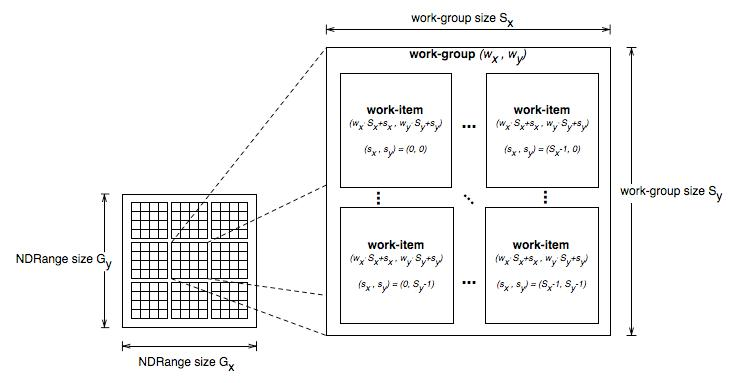
\includegraphics[width=0.8\textwidth]{figures/ndrange.jpg}
\caption{OpenCL NDRange \protect\footnotemark.}%
\label{rys:ndrange}
\end{figure}
\footnotetext{Źródło: http://www-igm.univ-mlv.fr/~dr/XPOSE2008/CUDA\_GPGPU/opencl\_threads.jpg}
Obszar NDRange jest metodą służącą do organizacji pamięci i zaplanowania zadań w architekturze OpenCL. NDRange to jedno-, dwu- lub trójwymiarowa przestrzeń. Jest ona podzielona na grupy robocze. Każda grupa posiada swój indeks, po którym można określić jej pozycję w przestrzeni. Każdy ciąg instrukcji, stanowiący odrębne zadanie kernela, dysponuje unikalnym globalnym numerem identyfikacyjnym a także unikalnym lokalnym numerem identyfikacyjnym wewnątrz każdej z grup.  \\
Tak podzielona przestrzeń wynika z architektury OpenCL. Dzięki identyfikatorom można skorzystać z bariery lokalnej, czyli wstrzymać wykonywanie kolejnych operacji dla zadań w ramach danej grupy roboczej do momentu zsynchronizowania operacji na wszytkich zadaniach grupy.

\section{Zarządzanie pamięcią w OpenCL}
W OpenCL używane są wymienione niżej cztery przestrzenie pamięci.
\begin{enumerate}
  \item Pamięć globalna - wszystkie wątki w grupach roboczych posiadają pełen dostęp (zapis i odczyt) do tej pamięci. Jest największym dostępnym obszarem pamięci jednak oferuje najwolniejszy dostęp
  \item Pamięć prywatna - dostęp do pamięci jedynie dla zadania, które zaalokowało pamięć podczas wykonywania danej instancji kernela.
  \item Pamięć lokalna - wszystkie wątki w danej grupie roboczej posiadają pełen dostęp do pamięci, jednak jest ona nieosiągalna dla wątków z innych grup. Możliwe jest zmapowanie obszaru pamięci globalnej na pamięć lokalną w celu uzyskania przyspieszonego czasu dosępu, jednak nie jest to wspierane przez wszystkie urządzenia.
  \item Pamięć stała. W tej kategorii pamięci przechowywane są stałe wartości podczas wykonania całej operacji kernela. Jest ona inicjalizowana przez hosta.
\end{enumerate}

\section{Urządzenia wykorzystane do testów}
\subsection{NVIDIA GTX 760}
Do testów została wykorzystana karta NVIDIA GeForce GTX 760, przedstawiona na rysunku 2.3. \\
\begin{figure}[h]
\centering
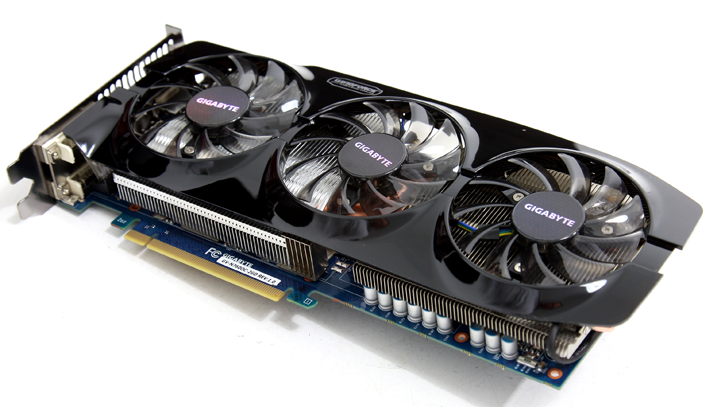
\includegraphics[width=0.8\textwidth]{figures/gtx.png}
\caption{NVIDIA GeForce GTX 760 \protect\footnotemark.}%
\label{rys:NVIDIA GeForce GTX 760}
\end{figure}
\footnotetext{Źródło: http://www.guru3d.com/articles-pages/geforce-gtx-760-gigabyte-windforce-review,1.html}
Karta została wyposażona w 1152 rdzeni CUDA (OpenCL uznaje je jako elementy przetwarzające) zebranych w 32 jednostkach obliczeniowych. Każdy z rdzeni jest taktowany zegarem o częstotliwości 1085 MHz. Maksymalna wydajność karty podczas obliczeń podwójnej precyzji wynosi 94 GFLOPsów (tysięcy operacji zmiennoprzecinkowych na sekundę), zaś podczas obliczeń w pojedynczej precyzji 2258 GFLOPSów. Karta została wyposażona w 2GB pamięci RAM typu GDDR5, taktowanej efektywną prędkością 1502 MHz. Wspiera standard OpenCL w wersji 1.2 oraz 2.0. \footnotemark[4]\\
\newpage
\subsection{Intel\textregistered Core\texttrademark i5-3570K}
Do testów został wykorzystany również procesor Intel\textregistered Core\texttrademark i5 model 3570K przedstawiony na rysunku 2.4. 
\begin{figure}[h]
\centering
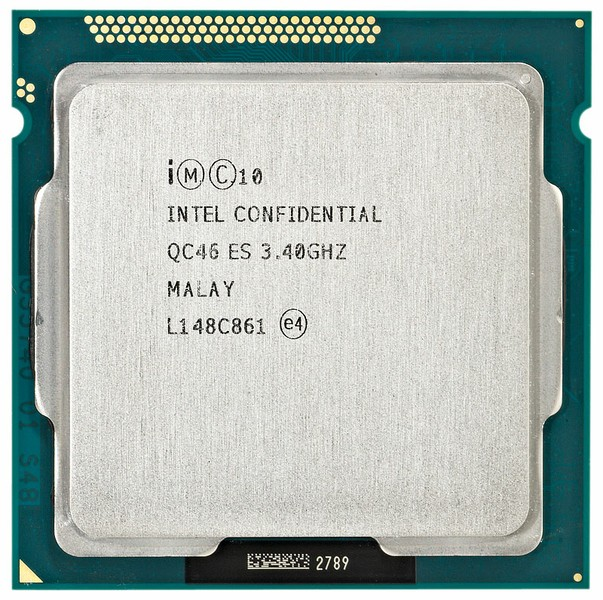
\includegraphics[width=0.3\textwidth]{figures/intel.jpg}
\caption{Intel\textregistered Core\texttrademark i5-3570K \protect\footnotemark.}%
\label{rys:Intel Core i5-3570K}
\end{figure}
\footnotetext{Źródło: http://www.chip.pl/images/testy/podzespoly-pc/procesory/intel-core-i5-3570k/56068.jpg/image\_preview}
\\Posiada cztery rdzenie, które mogą na raz przetwarzać maksymalnie do czterech wątków. Procesor pracuje w zakresie częstotliwości 3.4 - 3.8 GHz. Jest to urządzenie zrealizowane w technologii 22nm o archtekturze noszącej nazwę Ivy Bridge. Posiada on 128 KB pamięci L1 Data Cache oraz 128 KB L1 Instruction Cache. Urządzenie to wspiera standard OpenCL w wersji 1.2\footnote{Źródło: http://ark.intel.com/pl/products/65520}.
